\chapter*{Ejercicio 9}
\addcontentsline{toc}{chapter}{Ejercicio 9}
A partir del filtro de la Figura \ref{fig:e9filtro} se obtuvo la ecuación de diferencias

\begin{equation}
    y(nT)=0.5 \cdot x(nT -2T) + \alpha \cdot y(nT-T) + \beta \cdot y(nT-2T)
\end{equation}

\begin{figure}[ht]
    \centering
    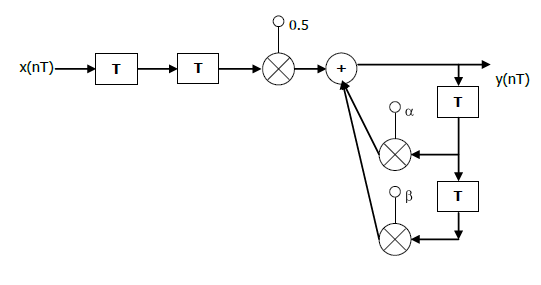
\includegraphics{ej9.png}
    \caption{Filtro Recursivo de Segundo Orden}
    \label{fig:e9filtro}
\end{figure}

Usando MATLAB, se computaron las respuestas al impulso y al escalón para los siguientes conjuntos de valores y sus resultados se muestran en sus respectivas figuras:
\begin{enumerate}
    \item \(\alpha  = 1 \qquad \beta = -1/2 \) (Figura \ref{fig:9a})
    \item \(\alpha  = 1/2 \qquad \beta = -1/8\) (Figura \ref{fig:9b})
    \item \(\alpha  = 5/4 \qquad \beta = -25/32 \) (Figura \ref{fig:9c})
\end{enumerate}

\begin{figure}
    \centering
    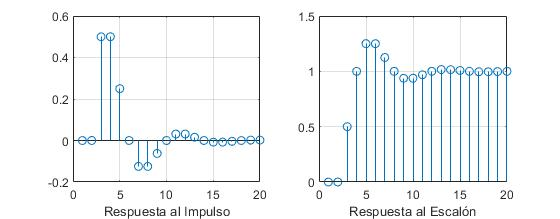
\includegraphics[width=\linewidth]{sim9a.jpg}
    \caption{Resultado de la simulación con $\alpha=1$ y $\beta=-1/2$}
    \label{fig:9a}
\end{figure}

\begin{figure}
    \centering
    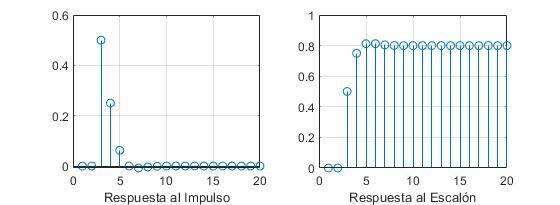
\includegraphics[width=\linewidth]{sim9b.jpg}
    \caption{Resultado de la simulación con $\alpha=1/2$ y $\beta=-1/8$}
    \label{fig:9b}
\end{figure}

\begin{figure}
    \centering
    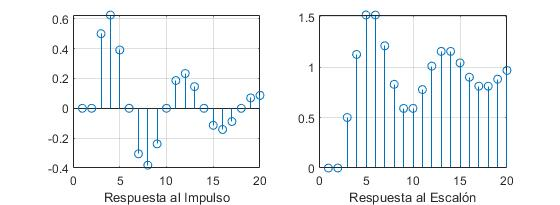
\includegraphics[width=\linewidth]{sim9c.jpg}
    \caption{Resultado de la simulación con $\alpha=-5/4$ y $\beta=-25/32$}
    \label{fig:9c}
\end{figure}

A partir de los resultados obtenidos de las simulaciones, se determinó la frecuencia de oscilación de los tres sistemas.

En el sistema 1, se puede observar que el período de oscilación es de $8 nT$. Por lo tanto, la frecuencia de oscilación será de $f=\frac{1}{8nT}$.

En el sistema 2, no se observan oscilaciones, por lo tanto no se puede determinar una frecuencia de oscilación.

Por último, en el sistema 3 se observa de la respuesta al impulso que el período de oscilación es de $8nT$; por lo tanto, la frecuencia de oscilación será de $f=\frac{1}{8nT}$.

Para el sistema del caso a, se puede estimar su respuesta en frecuencia intercambiando ingresando una señal sinusoidal, $x(nT) = e^{j\omega nT}$ en lugar de un impulso e iterando los resultados con distintos valores de $\omega$. Analíticamente, dado que se obtuvo la respuesta al impulso de este sistema, si a esta se le aplica la convolución con esta señal sinusoidal, también puede obtenerse su respuesta en frecuencia.